\chapter{\Edgeworth{} Usability Evaluation}

\section{Definitions}
\label{sec:definitions}

In the discussion of translation problems, \cref{chp:edgeworth} uses terms such as ``instance,'' ``noninstance,'' ``near hit,'' and ``near miss.'' To standardize the terminologies in this appendix, I give some definitions here.

Given a set of mathematical statements describing logical entities and their relationships, a diagram can be associated with them in one of the following ways:

\vspace{0.5em}
\begin{figure}[h]
\begin{minipage}[b]{0.48\linewidth}
$\bullet$ \textbf{Example}: the diagram represents the math statements, \ie all the statements hold true in the diagram. 
    \vspace{3pt}
    
$\bullet$ \textbf{Counterexample}: the diagram clearly violates the math statements, \ie one or more statements are false in the diagram.
    \vspace{3pt}
    
$\bullet$ \textbf{Positive edge case}: the diagram is an example of the math statements, but contains extraneous entities and/or more specialized relationships. 
    \vspace{3pt}
    
$\bullet$ \textbf{Negative edge case}: the diagram is a counterexample, but only requires a few changes to become an example.
\end{minipage}
\hfill
\begin{minipage}[b]{0.45\linewidth}
    \centering
    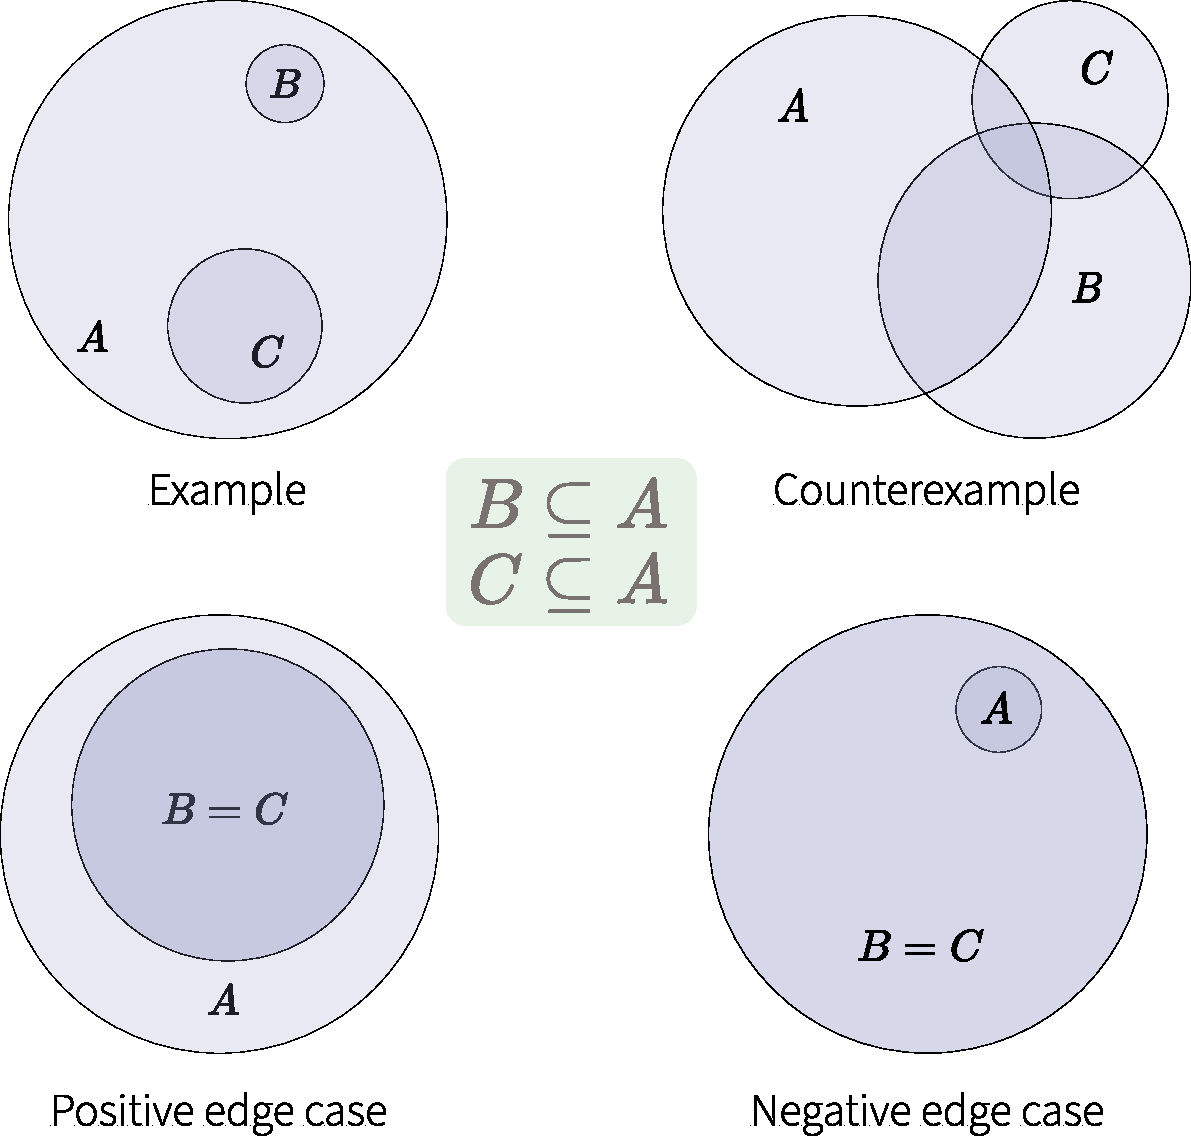
\includegraphics[width=\textwidth]{assets/appendix/definitions-examples.pdf}
\end{minipage}
\end{figure}

% While distinguishing between examples and counterexamples is often straightforward, identifying edge cases can depend on the context. For instance, the counterexamples in the figure above both violate all math statements, but the lower-right diagram can be considered an edge case because one can swap the labels $A$ and $B$ to make it an example. 

\section{Summary of proposed work}

\subsection{Programming-by-example workflow}


\begin{figure}
    \centering
    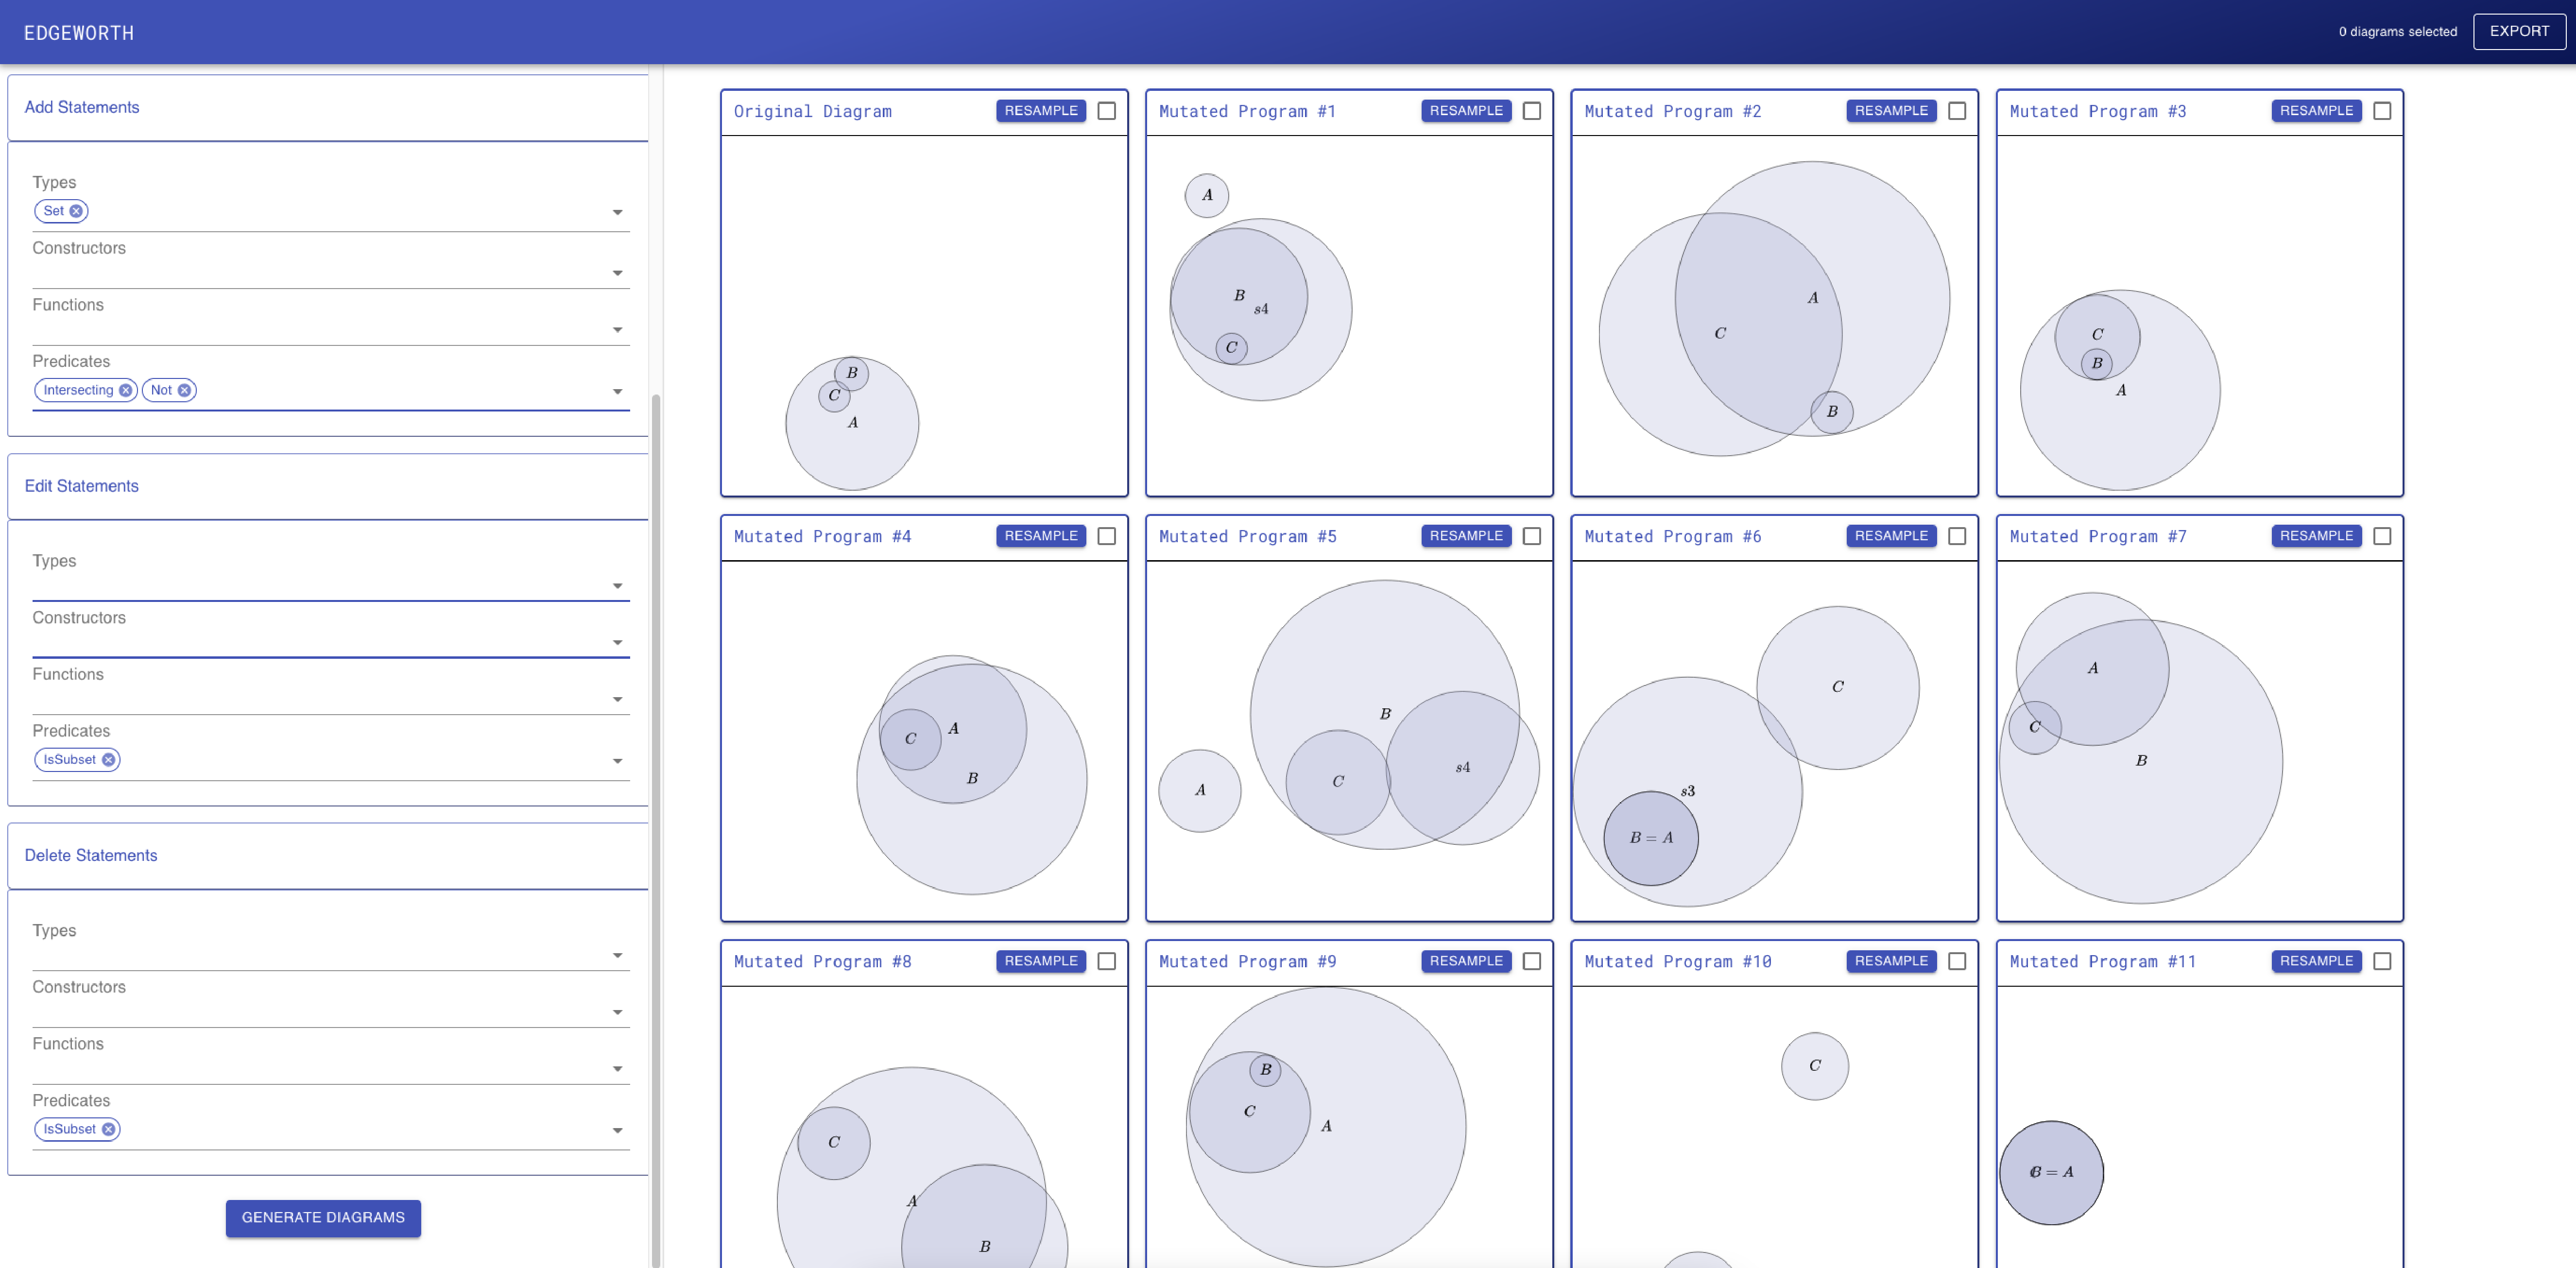
\includegraphics[width=\linewidth]{assets/appendix/edgeworth-bad-output.pdf}
    \caption{A screenshot of the \Edgeworth interface, after generating examples for a translation problem focusing on improper subsets. Because of the configuration, pool of mutant diagrams aren't suitable for this problem.}
    \label{fig:edgeworth-bad-output}
\end{figure}


With the \Edgeworth mutator, the primary mode of interaction is configuration-based: the author creates a mutator configuration and the mutator generates a set of diagrams. When these diagrams don't satisfy the needs of the author (\eg missing counterexamples that are important for an educational goal), the author can only edit the configuration again and hope to get better ones. In short, the quality of \Edgeworth-generated diagrams are sensitive to the configuration. 

For example, suppose an author would like to create translation problems that test students' knowledge of improper subsets, especially the fact that if $A \subseteq B$, $A = B$ is allowed. Using the \Edgeworth mutator, the author first creates a prompt \Substance program:

\begin{verbatim}
Set A, B, C
IsSubSet(B, A)
IsSubset(C, A)
\end{verbatim}

Not familiar with how program mutator works, the author picks a few options in the configuration interface and clicks ``Generate Diagrams.'' Ideally, \Edgeworth should generate a set of examples of the subset relations that include the edge cases of $A = B$, $A = C$, or $B = C$, and counterexamples of $B \not\subseteq A$ or $C \not\subseteq A$. 

However, the output from \Edgeworth seems too random (\cref{fig:edgeworth-bad-output}). There are useful counterexamples, but none of the diagrams include edge cases such as:
\begin{verbatim}
Set A, B, C
IsSubSet(B, A)
IsSubset(C, A)
Equal(B, C)
\end{verbatim}

In other words, without intimate knowledge of how the \Edgeworth mutator is configured, the author cannot express their intent easily. In this case, it's much more natural to write a few examples from scratch, or manually make slight tweaks to examples in the mutant pool. I propose to \textbf{create a programming-by-example (PBE) workflow, where the author manually creates or edits a few diagrams, and \Edgeworth generates more diagrams with similar properties.}

Using this workflow for the example above, the author can manually create a few examples by directly editing the prompt program. In this case, the author adds the \sub{Equal(B, C)} predicate. Their intent is to include the edge case of improper subsets in this problem, where some of the subset relations are actually equality. \Edgeworth generates a set of similar examples that add \sub{Equal} predicates with existing identifiers in different ways. 

\vspace{10pt}
\begin{figure}[h]
    \centering
    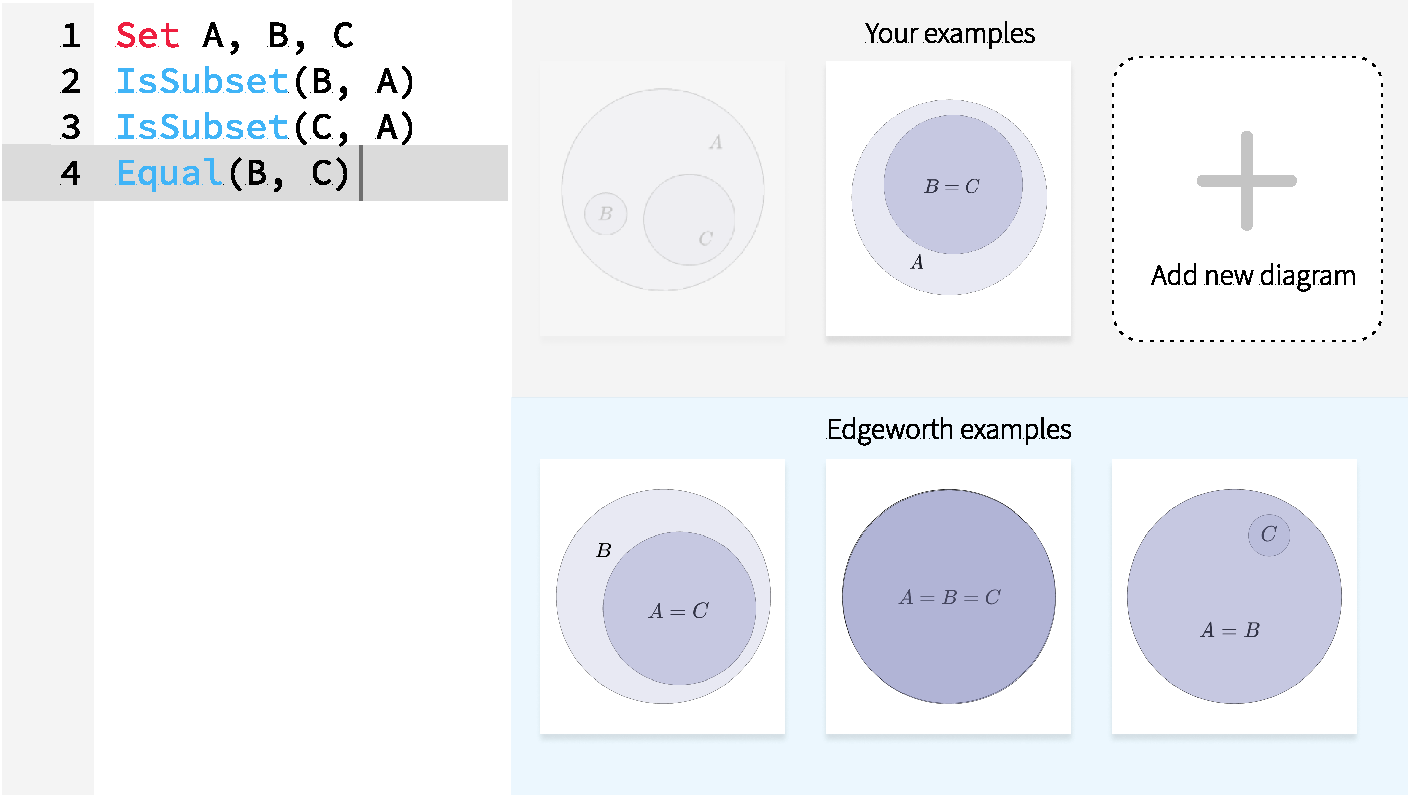
\includegraphics[width=0.8\linewidth]{assets/appendix/synthesis-driven-workflow.pdf}
    % \caption{Caption}
    % \label{fig:my_label}
\end{figure}
\vspace{10pt}

The addition of \sub{Equal(B, C)} is effectively a user-generated mutation, and \Edgeworth needs to understand this mutation to generate similar instances. To do so, the \Edgeworth synthesizer matches a series of author edits to predefined mutations. Once the synthesizer finds a mutation path that describes the author edit, it can then inform the mutator to generate examples with similar properties (\ie including the edge case of equal sets). Using this workflow, the author can rapidly author diagrams that belong to a particular category in the translation problem. For example, the problem below has diagrams that include set equalities as correct answers, and diagrams that violate one or both subset relations as incorrect answers.

\vspace{10pt}
\begin{figure}[h]
    \centering
    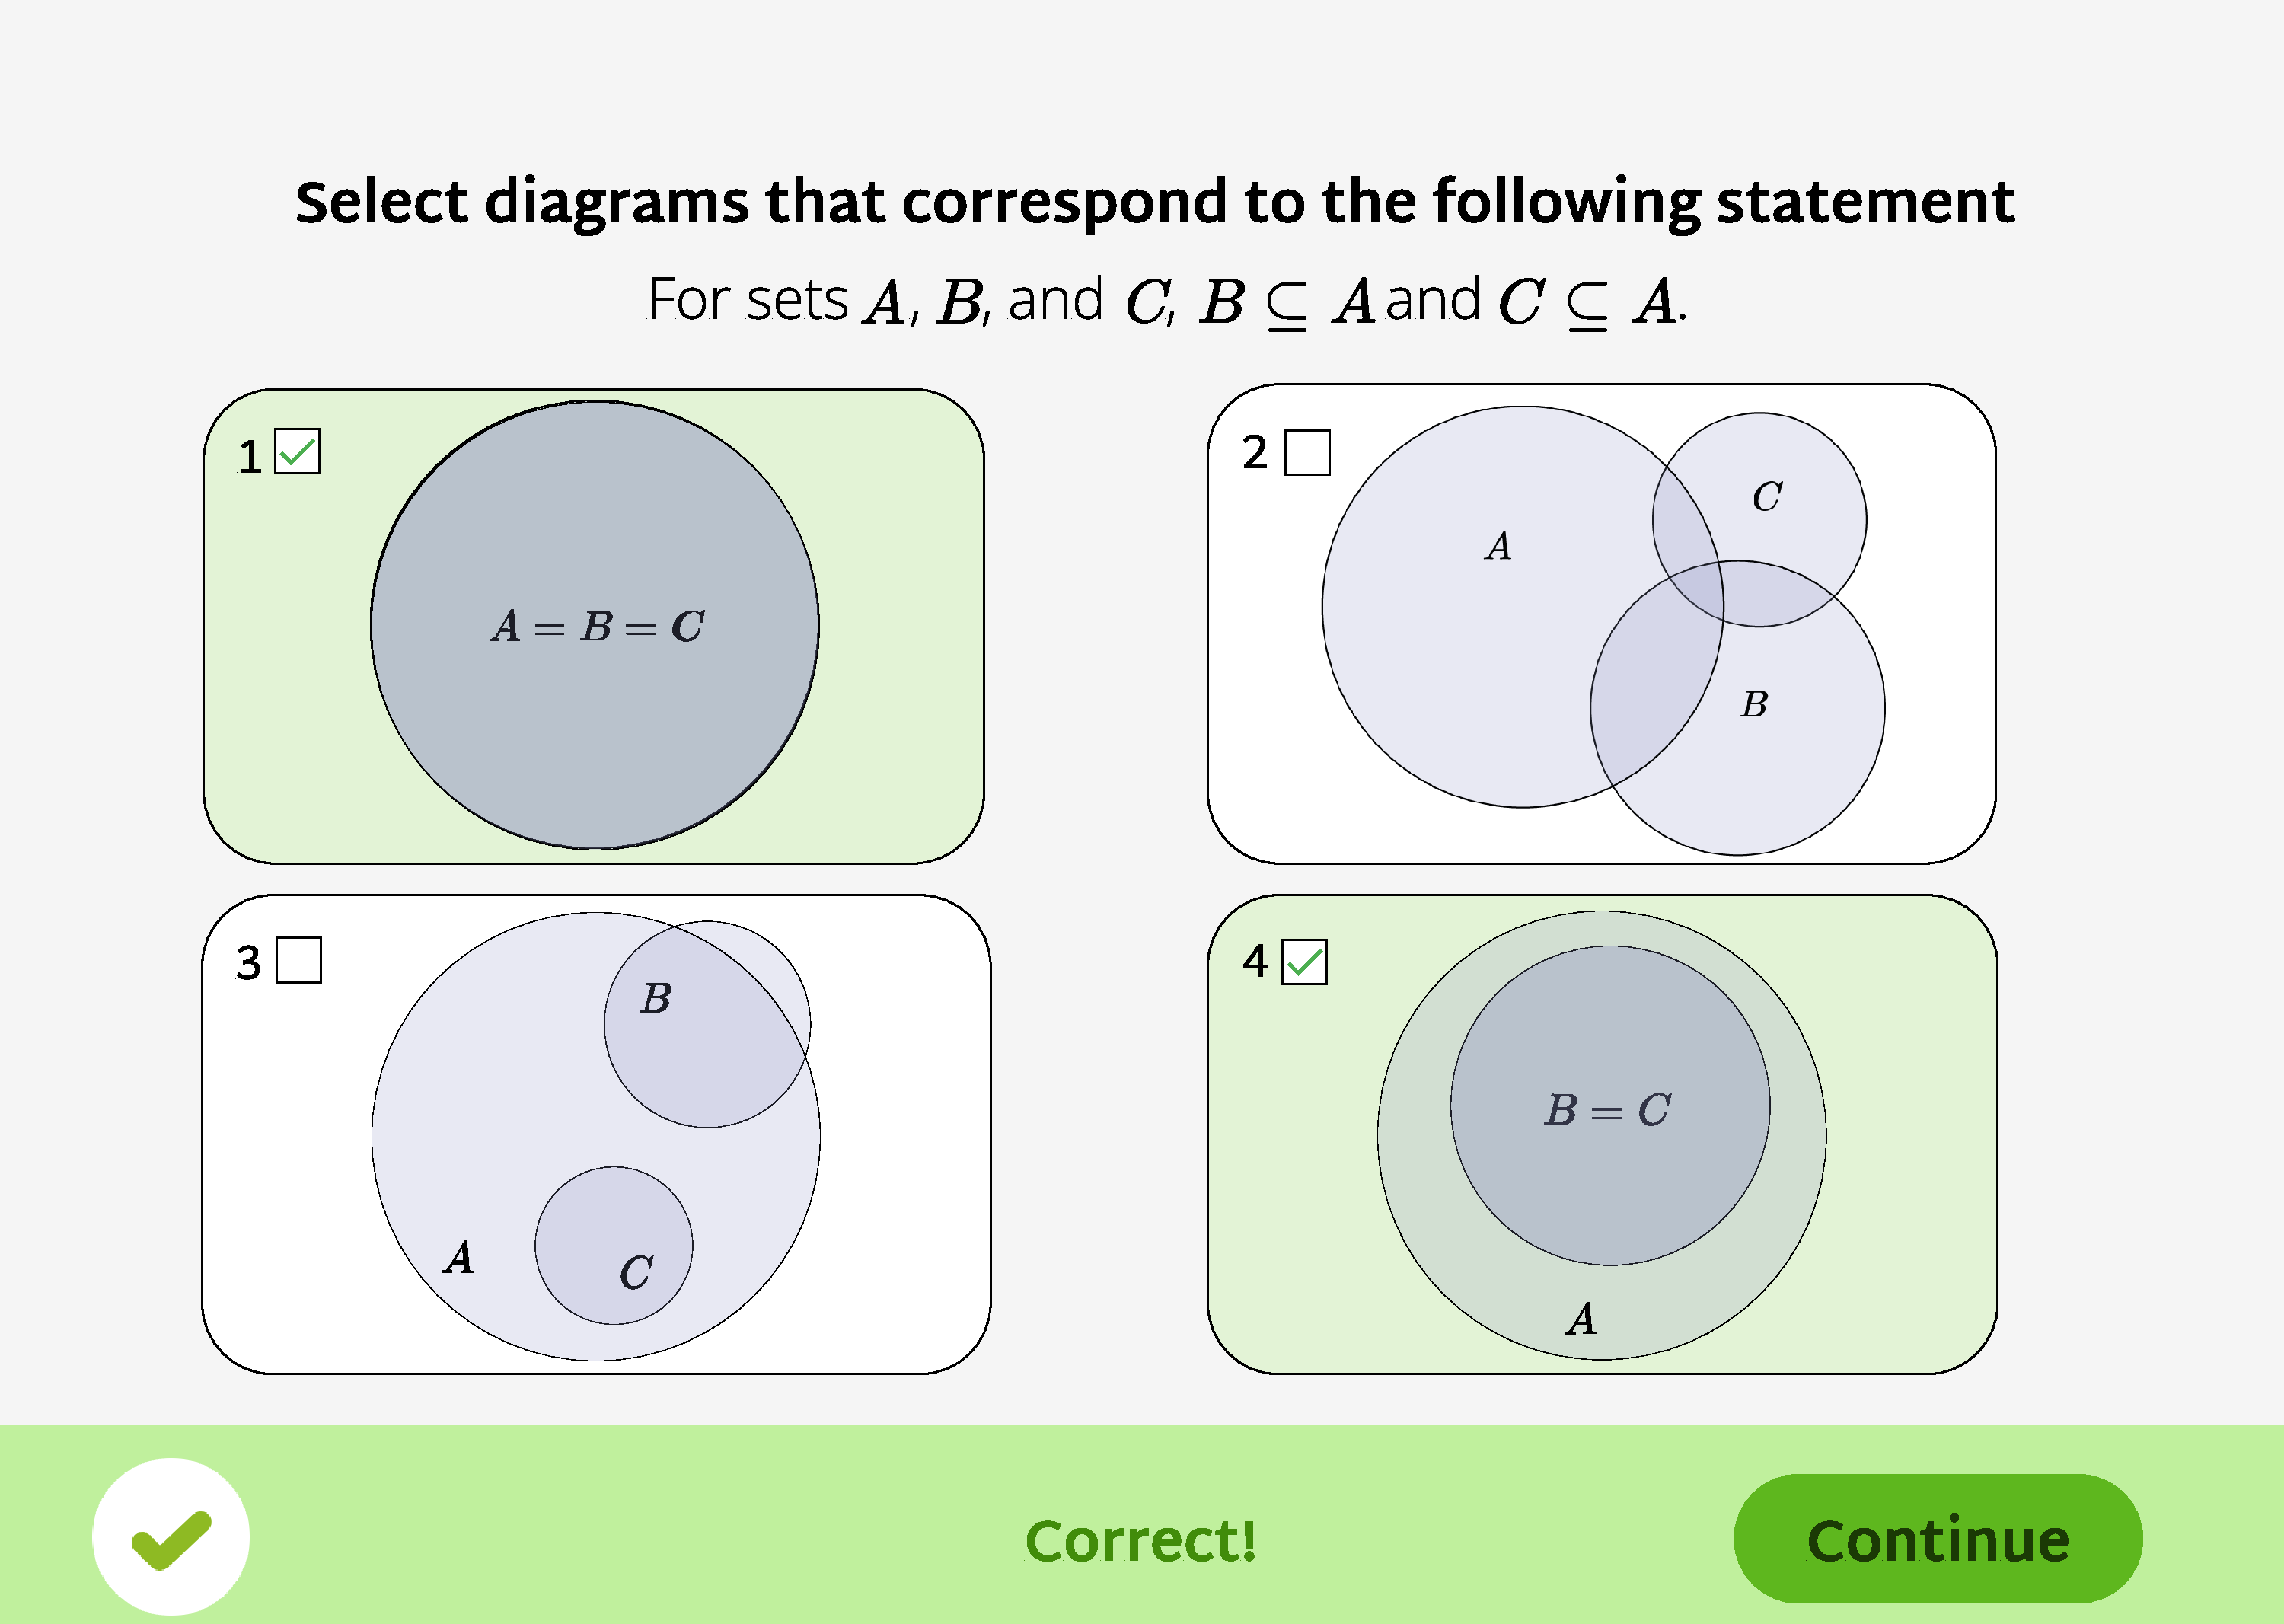
\includegraphics[width=0.8\linewidth]{assets/appendix/translation-problem-sets.pdf}
    % \caption{Caption}
    % \label{fig:my_label}
\end{figure}
\vspace{10pt}

\subsection{Automatic detection of examples and counterexamples}
\label{sec:autodetect}

One key application of \Edgeworth is generating translation problems with examples and counterexamples. Therefore, it's important for the system to understand whether a diagram is an example or counterexample of the prompt. However, the \Edgeworth mutator performs \Substance program mutations on the prompt without knowing if a mutant is semantically equivalent to the prompt. To address this, I propose to \textbf{automatically detect examples and counterexamples}.

One heuristic is cross-instance energy evaluation (CIEE) described in~\cref{sec:mutation}.  CIEE determines the distance between two \Substance programs by examining visual constraint satisfaction. 

Another approach is to provide the \Edgeworth mutator with more semantic information such that it generates examples and counterexamples by construction. Currently, none of the mutation operators carry any mathematical semantics because \Domain doesn't contain enough information. For instance, many mathematical predicates have reflexive, symmetric, transitive, and substitution properties, but \Domain only encodes basic type definitions. For a more precise notion of correctness, I plan to extend \Domain to model such properties, and use them in the \Edgeworth mutator, possibly together with CIEE, to generate higher quality mutants.  

\subsection{Hypotheses and research questions}

Comparing with related work discussed in \cref{sec:edgeworth-related}, \Edgeworth uniquely support scalable generation of diagrammatic translation problems in multiple domains. Therefore, in this section, I discuss hypotheses that cover the essential features of \Edgeworth such as the mutation-based approach and automatic detection of examples and counterexamples. For each hypothesis, I will also discuss further research questions to be investigated in the evaluation plan. 

\boxtext{\textbf{H1:} Given manageable effort in configuring the mutator, \Edgeworth can reliably generate examples and counterexamples for translation problems with relatively few mutants required.}

An effective translation problem needs to include both examples and counterexamples. Therefore, the technical approach of \Edgeworth---program mutations on \Substance code---must produce them reliably. To verify H1, the following research questions need to be answered:

\begin{itemize}
    \item \textbf{R1.1}: How many mutants does \Edgeworth need to generate to obtain sufficient examples and counterexamples for translation problems?
    \item \textbf{R1.2}: How frequently does \Edgeworth succeed or fail at doing so?
\end{itemize}

The preliminary evaluation showed that the mutator configuration will affect the quality of the mutants. Therefore, I will also address the following research question on mutator configuration and will use the results to further investigate possible ways to lower the configuration burden, e.g. the programming-by-example workflow and changes to the configuration format.

\begin{itemize}
    \item \textbf{R1.3}: How much configuration effort is required to produce examples and counterexamples? 
\end{itemize}

\boxtext{\textbf{H2}: \Edgeworth makes translation problem authoring more efficient.}

The main goal of \Edgeworth is to improve the efficiency of translation problem authoring. To verify H2, the evaluation plan will answer:
\begin{itemize}
    \item  \textbf{R2.1}: Comparing with workflows that authors are using, can \Edgeworth shorten the authoring time of translation problems?
    \item  \textbf{R2.2}: Which aspect(s) of the authoring workflow does \Edgeworth simplify, and does \Edgeworth introduce new authoring difficulties? 
    \item  \textbf{R2.3}: Are authors more efficient using the configuration-based workflow or programming-by-example workflow?
\end{itemize}

Regardless of the answer to R2.1, meaningful results on R2.2 can provide more insights on how \Edgeworth's approach impacts the problem authoring experience. For instance, I postulate that \Edgeworth improves authoring efficiency by (1) simplifying the mechanics of diagram production and (2) reducing the author's effort to come up with examples and counterexamples. On the other hand, \Edgeworth's mutation-based approach may introduce new problems such as difficulties finding the right diagrams from the mutant pool and controlling the quality of examples. The automatic detection heuristics described above aim to mitigate these difficulties.

\boxtext{\textbf{H3}: \Edgeworth can automatically distinguish examples from counterexamples, and this feature helps authors find examples and counterexamples for translation problems.}

The effectiveness of translation problems depends on the choice of examples and counterexamples. I hypothesize that example generation/selection is a nontrivial activity that authors spend time doing, and computational support in \Edgeworth can help authors identify examples/counterexamples. Answering the following research questions will verify H3:

\begin{itemize}
    \item \textbf{R3.1}: Can \Edgeworth automatically detect examples, counterexamples, and edge cases with a reasonably high accuracy?
    \item \textbf{R3.2}: Do the detection results help authors identify potential answers to translation problems?
\end{itemize}


\section{Plan}

\subsection{Pilot usability evaluation}

To prepare the \Edgeworth prototype for evaluation, I will first evaluate the usability of \Edgeworth by recruiting authors to perform small authoring tasks with the \Edgeworth prototype. For example, the participants may be asked to author a simple diagrammatic translation problem. The goal of this pilot study is to identify missing features, usability problems, and opportunities for simplification. The study may include several rounds with increasingly high-fidelity prototypes. After each round, I will refine the design and implement the next prototype. Here are some possible high-level questions for the study:
\begin{itemize}
    \item What are the key design considerations for translation problem authoring? How do they fit with the features of \Edgeworth?
    \item How do authors prefer to work with \Edgeworth? When do they opt to write a configuration file and generate many diagrams? When do they use the by-example workflow? Do they mix the two workflows?
    \item How does the experience compare to their existing tools? How can \Edgeworth incorporate useful parts of them? 
\end{itemize}

\subsection{Technical evaluation of automated production of diagram problems}
\label{sec:case-study}

While the preliminary study (\cref{sec:edgeworth-prelim-eval}) shows some promise of \Edgeworth's approach, the data from this study is insufficient for investigating H1 and R1.1-3. In this study, I will investigate if \Edgeworth can reliably produce diagrams for translation problems (H1) by gathering richer data on its success rate, efficiency, and human effort. 

\subsubsection{Translation problem set} 

I will reproduce diagrammatic problems from the same geometry textbook~\cite{holtGeometry} used in \cref{sec:edgeworth-prelim-eval}. In the textbook, diagrammatic problems often require representational fluency but aren't presented as multiple-choice translation problems with diagrams as choices. I plan to start with the original set of 24 translation problems that were reframed from textbook problems, and potentially extend the dataset using the same methodology of reframing the problems. Each translation problem in the dataset will include (1) a textual prompt, (2) four diagrams, and (3) a \Substance prompt program.

\subsubsection{Data collection} 

The output of \Edgeworth may be sensitive to factors like randomness of mutation paths and quality of configuration. Therefore, for each of the translation problems in the dataset, I will use the configuration-based workflow (\cref{sec:mutation}) in \Edgeworth to produce multiple problem instances. Each valid problem instance is a multiple-choice translation problem with four diagrams comprised of examples, counterexamples, and edge cases of the problem prompt. The validity of problem instances is determined manually during the study. 

Each problem instance may take multiple trials of executing the mutator and editing the configuration. The authoring process for each problem instance will be screen-recorded and documented. \Edgeworth will also be instrumented to log data such as the following:

\begin{itemize}
    \item Mutator data: mutant diagrams and their mutation paths, number of mutant generated per trial.
    \item Execution history: configuration file per execution and mutants selected for the translation problem.
    \item Edit history of the configuration: edits to a configuration for a particular translation problem and changes to configuration schema between translation problems.
\end{itemize}

\subsubsection{Proposed methodology} 

For R1.1, I plan to count (1) the number of mutants generated over multiple trials to obtain a valid problem instance and (2) the number of mutants in the last successful trial. The average of (2) over all translation problems measures the reliability of \Edgeworth given a good configuration, whereas that of (1) factors in the human effort of authoring such a configuration. To answer R1.2, I will run \Edgeworth with the configuration of the last successful trial, and measure the success rate of producing valid problem instances. 

For R1.3, I will use the screen recording to measure the time-to-completion for each valid problem instance and also count trials-to-completion. These data may be subject to particular contexts in which I will run the study. To gain a more objective understanding of the complexity of configuration files, I will also measure the specificity of the configuration to help answer R1.3. As a base case, an empty configuration with defaults takes no human effort to author, and a configuration that selects many constructs from \Domain takes significantly more effort. I will use the edit history and the length of the resulting configuration file itself to measure configuration effort.

% As discussed in \cref{sec:definitions}, while it's straightforward to distinguish between examples and counterexamples
The validity of edge cases depends on the context of a particular translation problem.  For all of the problems, I will label examples, counterexamples, and edge cases, and document the context and my rationale.  In addition, I will recruit a geometry teacher to label a sample of the problems from the dataset. I will then calculate the inter-rater reliability of between my rating and the teacher rating to assess whether my rating agrees with expert judgments. 

Then, I will use \Edgeworth to perform automatic detection (\cref{sec:autodetect}) on all translation problems from this study, and compute inter-rater reliability between the manual labels and detection results. Along with the documented edge case decisions from the study, a high inter-rater reliability can provide more confidence that \Edgeworth can accurately detect positive and negative edge cases (R3.1). 

\subsection{Experimental evaluation of authoring efficiency}

This study is an authoring experiment that compares (1) \Edgeworth against existing authoring tools and (2) features of \Edgeworth (\eg configuration vs. PBD, auto-detection on/off). Participants will create diagrammatic translation problems using conventional drawing tools or \Edgeworth. For H2, this study quantitatively measures the efficiency with or without \Edgeworth, compare between configuration-based and PBD workflows, and gather qualitative data on how \Edgeworth improves and/or hinders translation problem authoring. For H3, this study will test within-subjects whether the automatic detection feature helps participants in distinguishing and generating examples and counterexamples. 

\subsubsection{Tasks}

All participants will be asked to complete 4 translation problem authoring tasks, each sampled from the case study dataset (see \cref{sec:case-study}). For each task, the participant will be given (1) an textual problem prompt and (2) an example diagram (\ie a correct response to the prompt). Participants will create 3 instances of this problem, each with two examples and counterexamples (12 diagrams in total). In the participant is using \Edgeworth, they will also be given (3) a \Penrose trio corresponding to the prompt. 

\subsubsection{Proposed methodology}

The participants will be divided into 3 groups, each group distinguished by the tool being used: 
\begin{itemize}
    \item Control group: a conventional drawing tool\footnote{During recruitment, we will survey the participants to find a common tool they know}, \eg Google Drawings
    \item \Edgeworth-config group: \Edgeworth with the configuration-based interface
    \item \Edgeworth-PBD group: \Edgeworth with the PBD interface
\end{itemize}
For both \Edgeworth groups, the automatic detection feature will be enabled for 50\% of the tasks. Below is an example of the study setup, where D indicates \Edgeworth with automatic detection and N without.

\begin{table}[h]
\centering
\begin{tabular}{l|cccccc}
                    & Task 1 & Task 2 & Task 3 & Task 4  \\ \hline
Control             &   -    &    -   &    -   &   -   \\ 
\Edgeworth-config 1 & N      & D      & D      & N   \\
\Edgeworth-config 2 & D      & N      & D      & N   \\
\Edgeworth-PBD 1    & D      & N      & N      & D   \\
\Edgeworth-PBD 2    & N      & D      & N      & D   \\
\end{tabular}
\end{table}
Between tasks, participants will be asked to explain how they came up with examples and counterexamples, identified useful edge cases, and interacted with the authoring tool. The study sessions will be recorded and transcribed. 

The recording and \Edgeworth data will be analyzed to measure the authoring time for each task. The total authoring time difference between the conventional drawing tool and \Edgeworth will be used to answer R2.1. The time difference between \Edgeworth-config and \Edgeworth-PBD will answer R2.3. I will also observe the relative time participants spend on writing configuration in \Edgeworth-config and \Substance code in \Edgeworth-PBD. This observation will provide an estimate of the overhead of each workflow. Finally, I will compare the time with or without automatic detection (R3.2). 

If participants do spend less time with automatic detection enabled, there may be two possible sources of this speedup: (1) they can filter down mutant diagrams in \Edgeworth more quickly, \ie less tool interaction; (2) \Edgeworth helps offload the effort in identifying examples and counterexamples, \ie less example ideation. Participants' answers between tasks will help us determine which of these reasons is dominant (R2.2).

The video recordings will be coded to identify challenges participants encounter in both the conventional drawing tool and configuration-based or PBD \Edgeworth (R2.2, R2.3), and how they interact with the automatic detection result (R3.2). 

\section{Milestones and timeline}

\cref{fig:timeline} shows a plan for the sequence of the proposed work mapped to a timeline.

\vspace{10pt}
\begin{figure}[h]
\begin{center}
\begin{ganttchart}[y unit title=0.4cm,
y unit chart=0.5cm,
x unit=0.32cm,
vgrid,hgrid, 
title label anchor/.style={below=-1.6ex},
title left shift=.05,
title right shift=-.05,
title height=1,
progress label text={},
bar height=0.7,
group right shift=0,
group top shift=.6,
group height=.3]{1}{40}
%labels
\gantttitle{Fall 22}{11} 
\gantttitle{Spring 23}{11} 
\gantttitle{Summer 23}{7} 
\gantttitle{Fall 23}{11} 
\\
%tasks
\ganttbar{Usability Pilot}{1}{1} \\
\ganttgroup{System Impl.}{1}{16} \\
\ganttbar{Config system}{1}{4} \\
\ganttbar{PBD system}{9}{16} \\
\ganttgroup{Technical eval.}{3}{12} \\
\ganttbar{Dataset}{3}{4} \\
\ganttbar{Experiment}{5}{8} \\
\ganttbar{Analysis}{9}{10} \\
\ganttbar{Writeup}{11}{12} \\
\ganttgroup{Experimental eval.}{12}{28} \\
\ganttbar{Authoring Pilot}{15}{16} \\
\ganttbar{IRB \& Design}{12}{16} \\
\ganttbar{Recruitment}{14}{16} \\
\ganttbar{Experiment}{17}{23} \\
\ganttbar{Analysis}{24}{25} \\
\ganttbar{Writeup}{26}{28} \\
\ganttgroup{Dissertation}{29}{40} \\
\ganttbar{Drafting}{29}{36} \\
\ganttmilestone{Defense}{40}
% \ganttbar{task 3}{9}{10} \\
% \ganttbar{task 4}{11}{15} \\
% \ganttbar[progress=33]{task 5}{20}{22} \\
% \ganttbar{task 6}{18}{19} \\
% \ganttbar{task 7}{16}{18} \\
% \ganttbar[progress=0]{task 8}{21}{24}

% %relations 
% \ganttlink{elem1}{elem2} 
% \ganttlink{elem3}{elem4} 
% \ganttlink{elem1}{elem5} 
% \ganttlink{elem3}{elem5} 
% \ganttlink{elem2}{elem6} 
% \ganttlink{elem3}{elem6} 
% \ganttlink{elem5}{elem7} 
\end{ganttchart}
\end{center}
\caption{Timeline of \Edgeworth projects}
\label{fig:timeline}
\end{figure}